%!TEX root = matmul_wse.tex


\begin{figure}[b!]
  \centering
  \begin{subfigure}{0.70\columnwidth}
    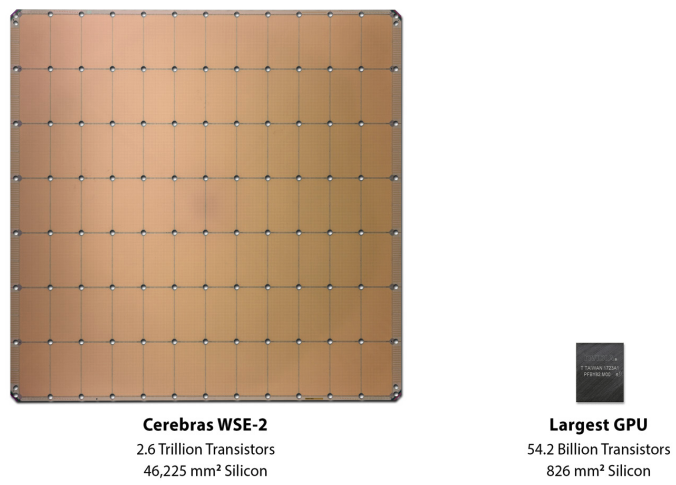
\includegraphics[width=\linewidth]{figures/wse2_vs_gpu.png}
  \end{subfigure}
  \caption{The Cerebras WSE-2 and the largest Graphics Processing Unit in comparison.}
  \label{fig:wse2_vs_gpu}
\end{figure}

The CS-2 is a system solution that consists of innovations across three dimensions: a) the second generation Cerebras Wafer Scale Engine (\wse) — the industry’s largest and only multi-trilliontransistor processor, b) the Cerebras System and c) the Cerebras software platform.
%
\wse is the processor at the heart of the CS-2, which is the largest chip ever built, as demonstrated in Figure~\ref{fig:wse2_vs_gpu}.
%
It is the industry’s only multi-trillion transistor processor, and contains more cores, more local memory, and more fabric bandwidth than any chip in history.
%
This enables fast, flexible computation at lower latency and with less energy.

The \wse covers 46,255 square millimeters — 56 times larger than the largest graphics processing unit.
With 850,000 cores, 40 Gigabytes of on-chip SRAM, 20 petabytes/sec of memory bandwidth, and 220
petabits/sec of interconnect bandwidth, the WSE-2 contains 123 times more compute cores, 1,000 times
more high-speed on-chip memory, 12,862 times more memory bandwidth and 45,833 times more fabric
bandwidth than its graphics processing competitor. In effect, it provides the compute capacity of an entire
cluster in a single chip, without the cost, complexity, and bandwidth bottlenecks involved with lashing
together hundreds of smaller devices. A summary of the comparison is shown in Figure~\ref{fig:wse2_vs_a100}.

\begin{figure}[t!]
  \centering
  \begin{subfigure}{0.90\columnwidth}
    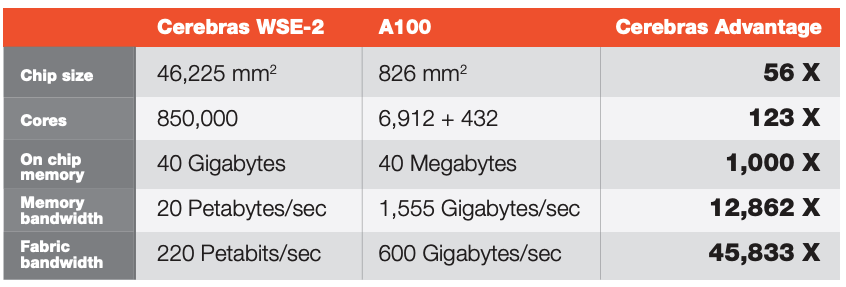
\includegraphics[width=\linewidth]{figures/wse2_vs_a100.png}
  \end{subfigure}
  \caption{Overview of the magnitude of advancement made by the Cerebras WSE-2}
  \label{fig:wse2_vs_a100}
\end{figure}



\begin{figure}[b!]
  \centering
  \begin{subfigure}{0.90\columnwidth}
    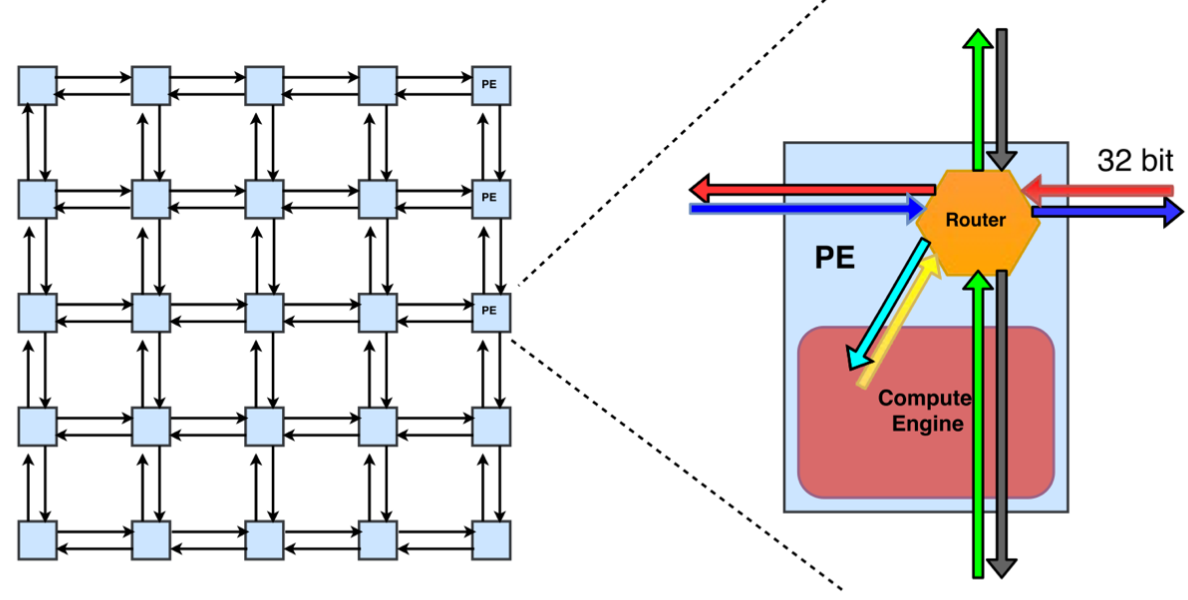
\includegraphics[width=\linewidth]{figures/pe.png}
  \end{subfigure}
  \caption{\wse organizations}
  \label{fig:pe}
\end{figure}



More details, the Cerebras Swarm communication fabric creates a massive on-chip network that delivers breakthrough bandwidth and low latency, at a fraction of the power draw of traditional communication techniques that are used to aggregate servers of graphics processing units into large clusters.
%
Swarm connects all 850,000 cores on the Cerebras \wse in a 2D-mesh with 220 Petabits/sec of
bandwidth (Figure~\ref{fig:pe} left).
%
Swarm provides a hardware routing engine to each of the cores and connects them with short wires optimized for bandwidth and low-latency. 
%
The resulting fabric supports single-word active messages that can be received by the cores without any software overhead, providing flexible, allhardware communication.
%
%
Each core is called processing element (PE), which is consist of a fabric router and a compute engine (CE), as shown in Figure~\ref{fig:pe} (right).


The router is a 5-port switch, with 1 port for each of the cardinal directions (North, South, East, and West), and one port for the CE.
%
The fabric router supports 24 virtual channels, called colors.
%
The switching unit is a wavelet, which consists of 32 data bits, one control bit, and 5 color bits. 
%
Wavelets are separated into two categories: control wavelets and data wavelets.
%
The fabric can receive a single wavelet per cycle from each of the 5 router ports and can send one wavelet per cycle on each of the 5 router ports.
%
The connection from fabric to compute engine is referred to as the “offramp”, and the connection from CE to fabric is called the "onramp".
%
Sitting at the boundary between the CE and the fabric are a set of queues and filters:
%
\begin{itemize}
  \item four filters, which can be used to selectively discard wavelets on the offramp;
  \item eight input queues, each of which is associated with a fabric color and serves as an extension of the fabric queue from the perspective of the CE;
  \item six output queues, holding wavelets generated by the CE until the fabric can accept them.
\end{itemize}


A CE is a simple compute core that runs instructions from memory.
%
Tasks are the primary unit of programming with only one task executing at a time.
%
There are two broad categories of tasks: wavelet-triggered tasks (WTTs) and local tasks. 
%
The scheduler can only choose to run tasks that are both unblocked and activated.
\begin{itemize}
  \item Wavelet-triggered tasks are activated by the arrival of wavelets, whether it be data wavelets or control 
  wavelets.
  %
  Data wavelets activate the data task associated with their color, while control wavelets activate the control tasks associated with the entry-point they store in bits 0 to 5 of the index field.
  \item Local tasks, on the other hand, can be activated by microthreads on completion or by FIFOs on pop or push.
  %
  They can also be activated using the {\it actvt} instruction.
\end{itemize}
%
Instructions that operate on vectors, which are described using data-structure registers (DSRs), are one of the important hardware features.
%
There are three main modes of execution: normal mode, single-step mode, and microthread mode.
\begin{itemize}
  \item In normal mode, vector instructions run until they complete.
  \item Single-step mode is similar to normal, but vector operands can be looped over so operations that require multiple instructions per-element can be executed.
  \item Microthread mode is quite different different and is a method of processing vectors that are received or transmitted on the fabric in a manner which does not require the processor to stall waiting for inputs or outputs to become available.
  %
  A microthreaded instruction is launched as part of a normal task, which then executes until it runs out of resources.
  %
  If it is unable to complete execution, it then effectively forks itself off to become an independent single-instruction task. 
  %
  Microthreads can be run concurrently with other tasks.
\end{itemize}

\begin{figure}[b!]
  \centering
  \begin{subfigure}{0.70\columnwidth}
    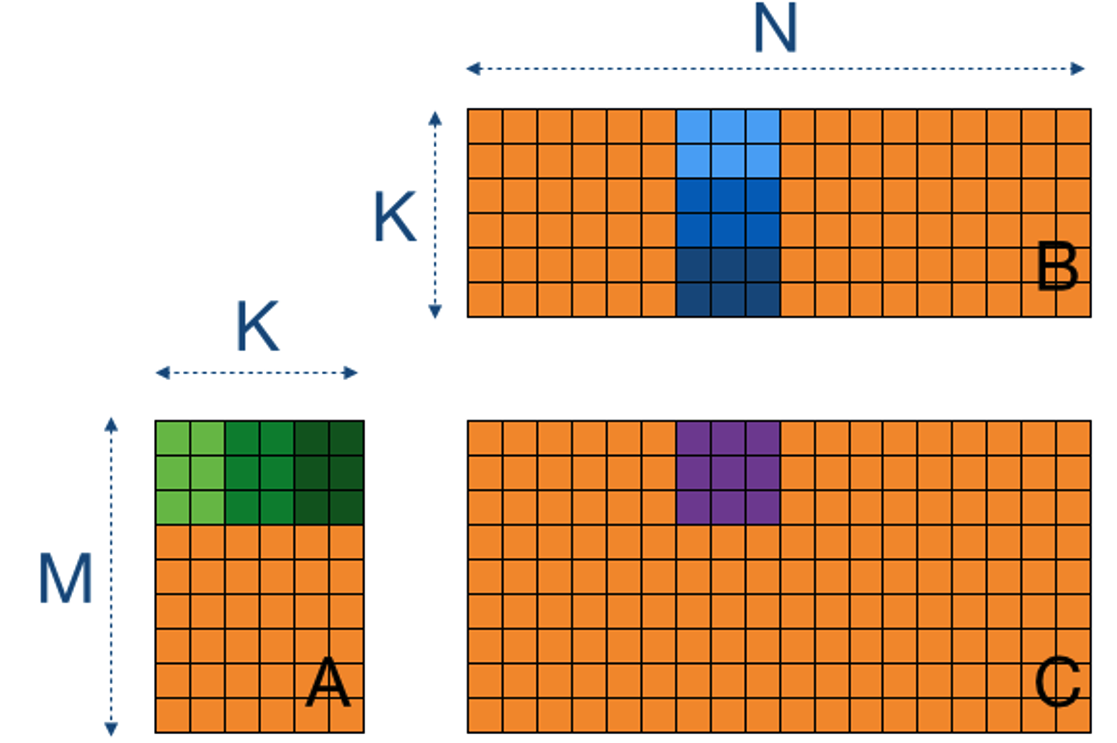
\includegraphics[width=\linewidth]{figures/gemm_overview.png}
  \end{subfigure}
  \caption{GEMM example}
  \label{fig:gemm_overview}
\end{figure}

Memory is a key component of every computer architecture. 
%
Memory closer to compute translates to faster calculation, lower latency, and better power efficiency for data movement. 
%
The \wse has 40 Gigabytes of on-chip memory, all uniformly distributed alongside the cores, and 20 Petabytes/sec of memory bandwidth, i.e., each PE holds 48KB on-chip memory and reads/writes at the rate of 32 bits/cycle.